\chapter{Исследовательский раздел}
\label{cha:research}

В данном разделе привидены и проанализированы примеры работы реализованной программы.

\section{Примеры работы}

На рисунках 4.1, 4.2, 4.3, 4.4 показана работа программы с различными входными данными.

\begin{figure}[H]
\centering
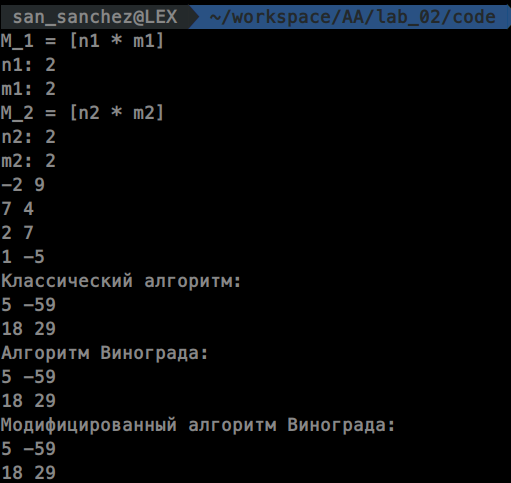
\includegraphics[scale=0.75]{./pict/wrk1.png}
\caption{Тест на случайных матрицах определенной длины}
\end{figure}
\begin{figure}[H]
\centering
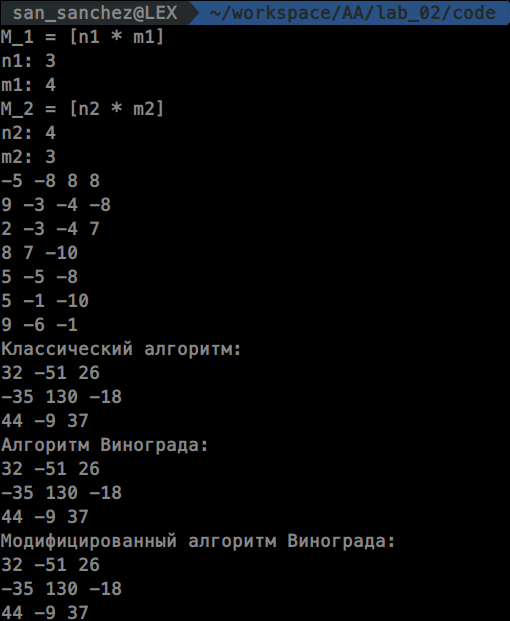
\includegraphics[scale=0.75]{./pict/wrk2.png}
\caption{Тест на случайных матрицах определенной длины}
\end{figure}
\begin{figure}[H]
\centering
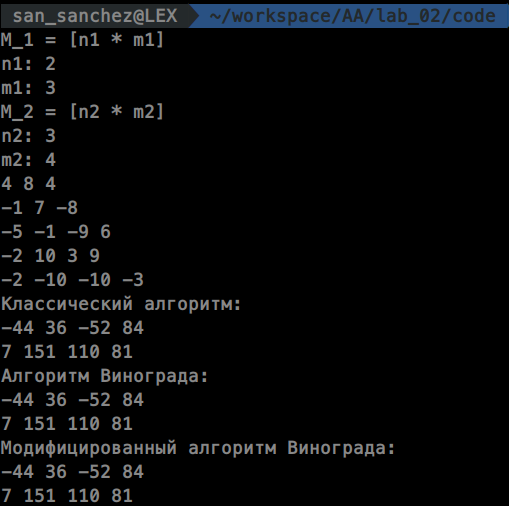
\includegraphics[scale=0.75]{./pict/wrk3.png}
\caption{Тест на случайных матрицах определенной длины}
\end{figure}
\begin{figure}[H]
\centering
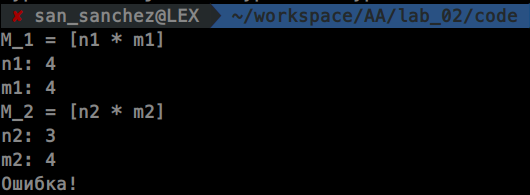
\includegraphics[scale=0.75]{./pict/wrk4.png}
\caption{Некорректный ввод}
\end{figure}

\newpage
\section{Эксперименты по замеру времени}
На графиках 6-7 представлено сравнение алгоритмов умножения матриц. 
	\begin{center}
        		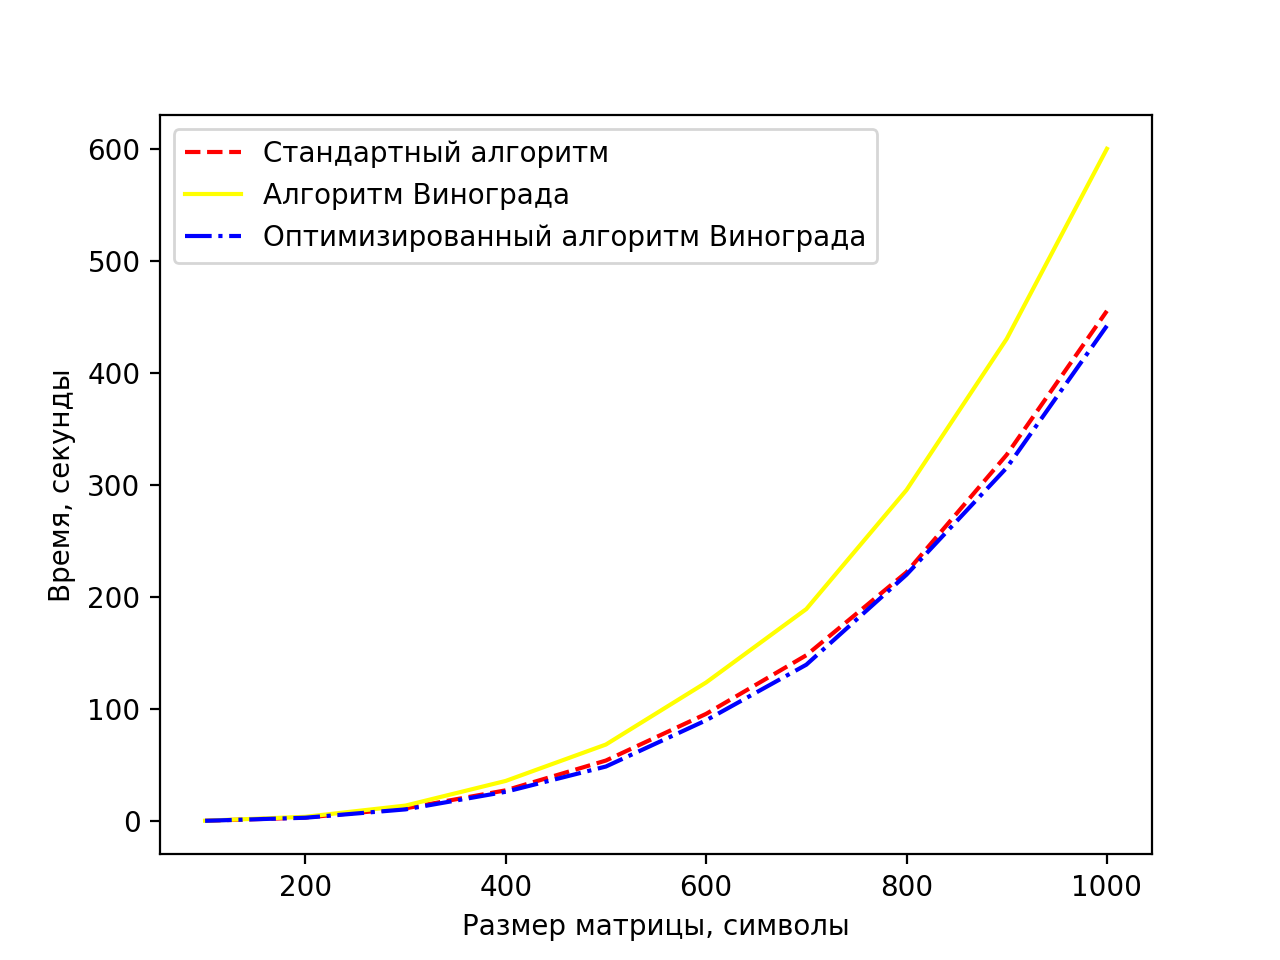
\includegraphics[scale = 1]{graph1} \\ Рис. 6 - Сравнение реализации алгоритмов нахождения произведения матриц при четных размерностях
	\end{center}
	
	\begin{center}
        		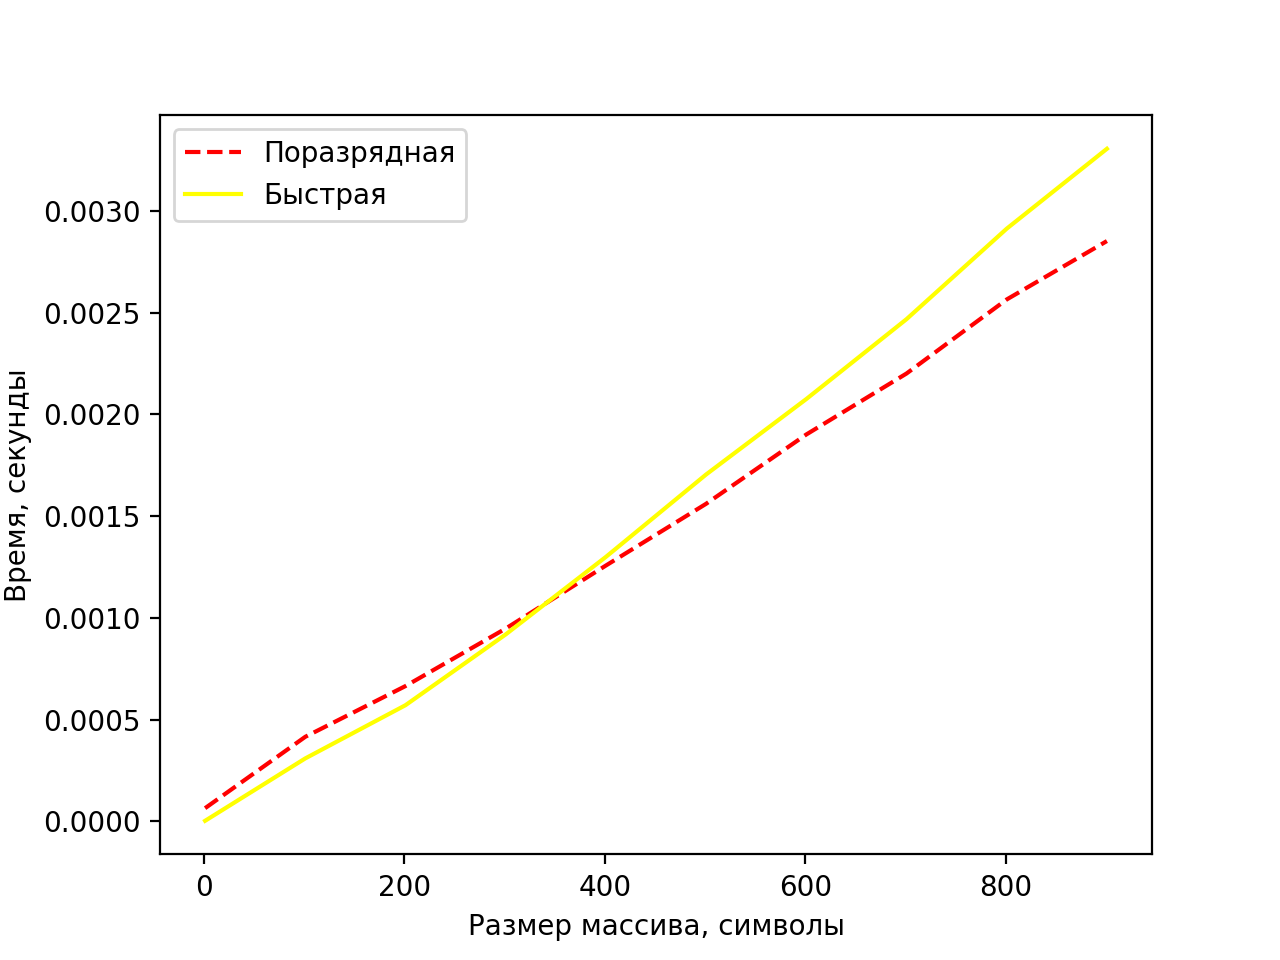
\includegraphics[scale = 1]{graph2} \\ Рис. 7 - Сравнение реализации алгоритмов нахождения произведения матриц при нечетных размерностях
	\end{center}
	
\section{Выводы}
	Как мы видим из графиков предположения о более быстрой работе Стандартного алгоритма по сравнению с Виноградом подтвердились, время вычислений меньше на 25\%. Но в плюсах использования алгоритма Винограда, это сокращение операции умножения. 
	Однако алгоритм Винограда с оптимизациями работает примерно также, как и стандартный, с этим связана оценка трудоемкости операции +=, оказывается в языке программирования Python эта операция выполняется гораздо дольше обычного сложения и присваивания.
	Также при сравнении работы для лучших случаев у Винограда (лучшие при четном размере матрицы) и худших (при нечетном) разница не значительна. 
\pagebreak

